\section{Part A}

In this part we have chosen two companies that offer online services in order to perform \textbf{Passive Scanning} on their websites. The two companies are of different scales on purpose, so that we can spot differences in their security approach. The smaller company that we chose is \textbf{Chip 7}, a national electronics chain of stores, with an online shop. The bigger company is \textbf{Farfetch}, a multinational online clothing store.

\subsection{Chip 7}

\subsubsection{Whois}

The first thing we did for each company was to run \textbf{whois} with their domain in order to get more information about them:

\begin{figure}[ht!]
 	\centering
 	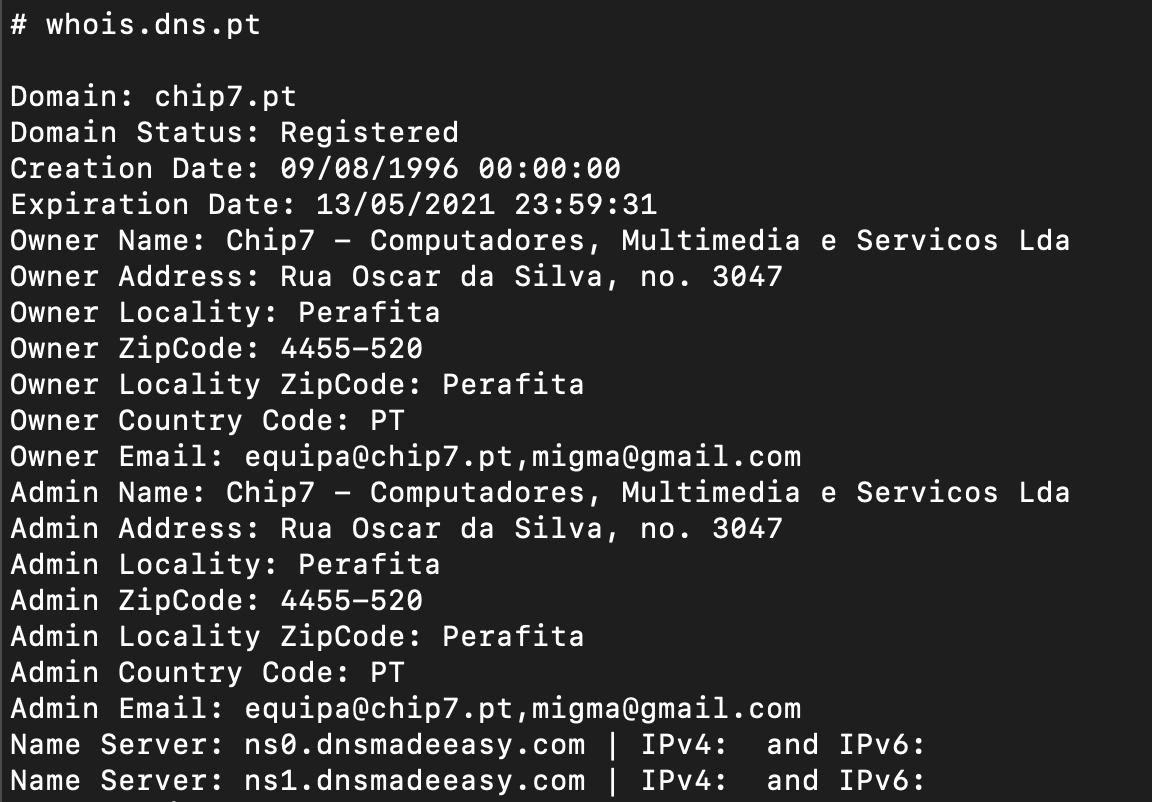
\includegraphics[width=0.9\linewidth]{img/whois1.png}
 	\caption{whois result}
\end{figure}
 
As we can see, we where able to obtain some information about the company, such as a physical address and a staff email.

Some useful information that hackers can be in the lookout for is, for example, the Expiration Date, Owner and Admin Emails, Owner and Admin Addresses and the Name Server. 

Being this a small company, it can happen that they forget to renovate the Domain, and the attacker is able to hijack it easily. The attacker can also be waiting for that date to expire. It can happen that the company takes some days to renew it. 

The Owner and Admin Emails can be used for fishing, an attacker can send emails with some link to a dubious site that asks for critical information or even download a malicious program that steals some other secrets.

In this case, the Owner and Admin Addresses are just a warehouse. That place can be the headquarters and can be used to perform Denial of Service attacks or vandalism on the part of the hackers, but being a franchise, it would not be a very efficient attack. Making a search on Google Maps it looks a place with some security too. If they weren't so careful, the addresses could have been the home of some element of the staff. That could be used for other kind of attack, like spying, take advantage of their private network vulnerabilities or even use the the email and social network of a naive element of the family to get some critical information useful for an attack or blackmail.


\subsubsection{Nslookup \& Whois}

The next step that we will take, is going to consist in retrieving the \textbf{IP Address} of the domain, and query whois again, using the obtained IP address. To retrieve the IP address of the domain, we will be using \textbf{nslookup}:

\begin{figure}[ht!]
 	\centering
 	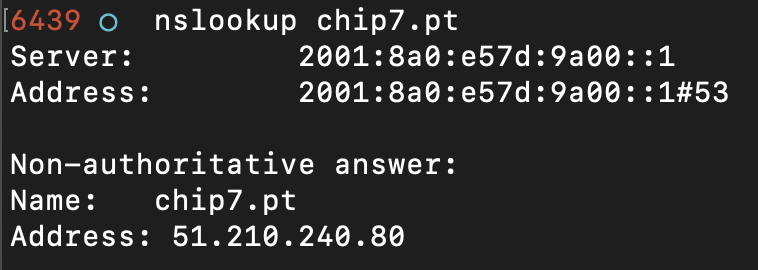
\includegraphics[width=.7\linewidth]{img/nsl1.png}
 	\caption{nslookup result}
\end{figure}

As we can see, we managed to get an \textbf{IP address}, and by querying \textbf{whois} with this new address we get the following:

\begin{figure}[ht!]
 	\centering
 	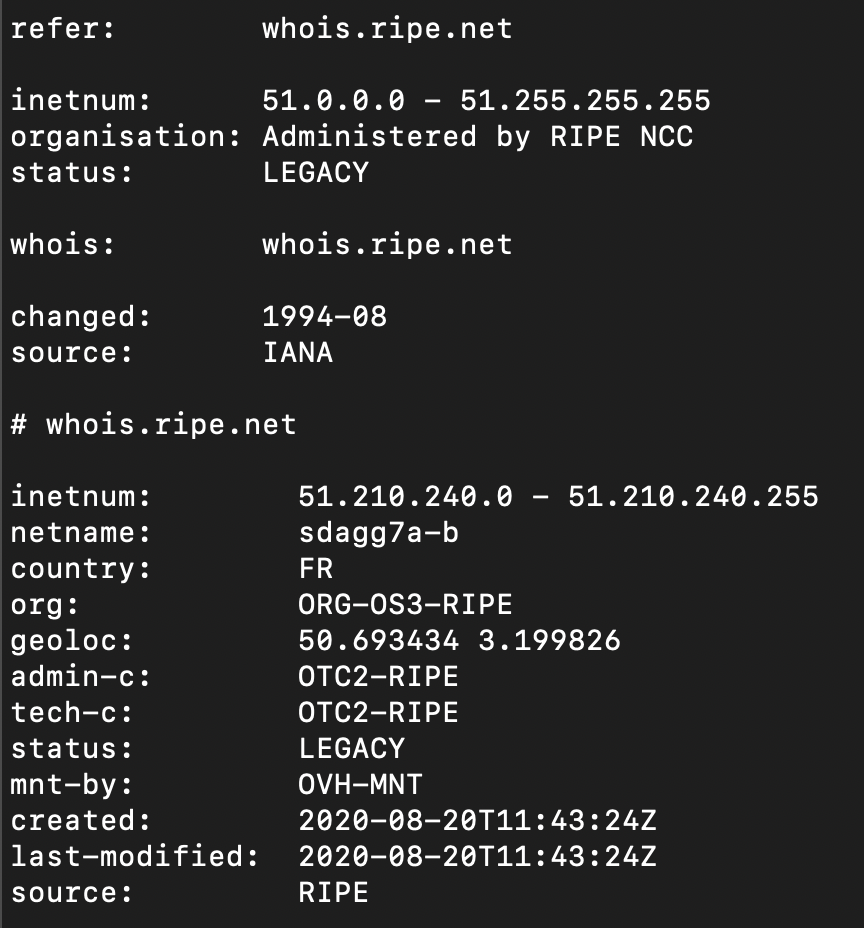
\includegraphics[width=.5\linewidth]{img/whois4.png}
 	\caption{whois result}
\end{figure}

Looking at the result we obtained, we discovered that the information is related to \textbf{RIPE}, a Network Coordination Centre. We also can use the \textit{mnt-by} attribute to have a slight idea that the \textbf{OVH}, which is a French cloud computing company that offers VPS, dedicated servers and other web services, may be the hosting provider for the company. Since we didn't get much information through the \textbf{IP address}, we changed our approach.

\subsubsection{Job offers}
We tried to get the technologies and tools used and other useful information, so we could try to get some vulnerabilities for them. For that purpose, we went on the lookout for active and past job offers. In the case of this company, we didn't find any information about this aspect, which makes us think that chip7 was careful with this topic. So, we went looking for a tool that would try to get that information just by inspecting the site. 

\subsubsection{BuiltWith}

As we are only using a passive search, a good idea would be use the \textbf{\href{https://builtwith.com/detailed/chip7.pt}{BuiltWith}} tool in order to know what technologies are used. 

As we can see from the figures below, we are able to see what kind of technologies are being used, such as \textbf{jQuery}, \textbf{PHP}, \textbf{PrestaShop}, \textbf{Vue}. We also know that they are using a \textbf{nginx} web server, and as we suspected. they are using \textbf{OVH} for hosting. Just with this tools we were able to uncover a lot of important information.

\begin{figure}[ht!]
 	\centering
 	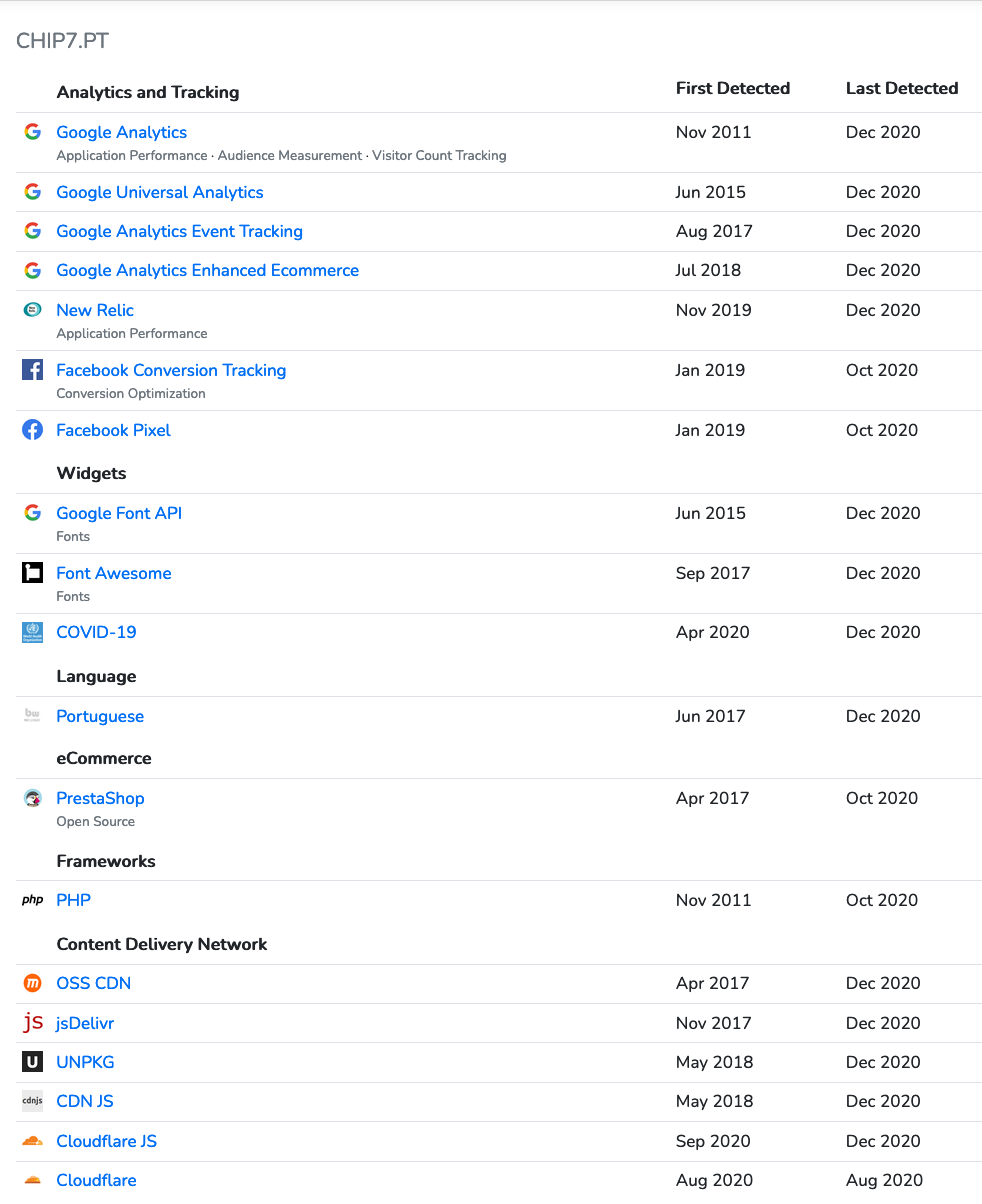
\includegraphics[width=.5\linewidth]{img/builtwith1.png}
 	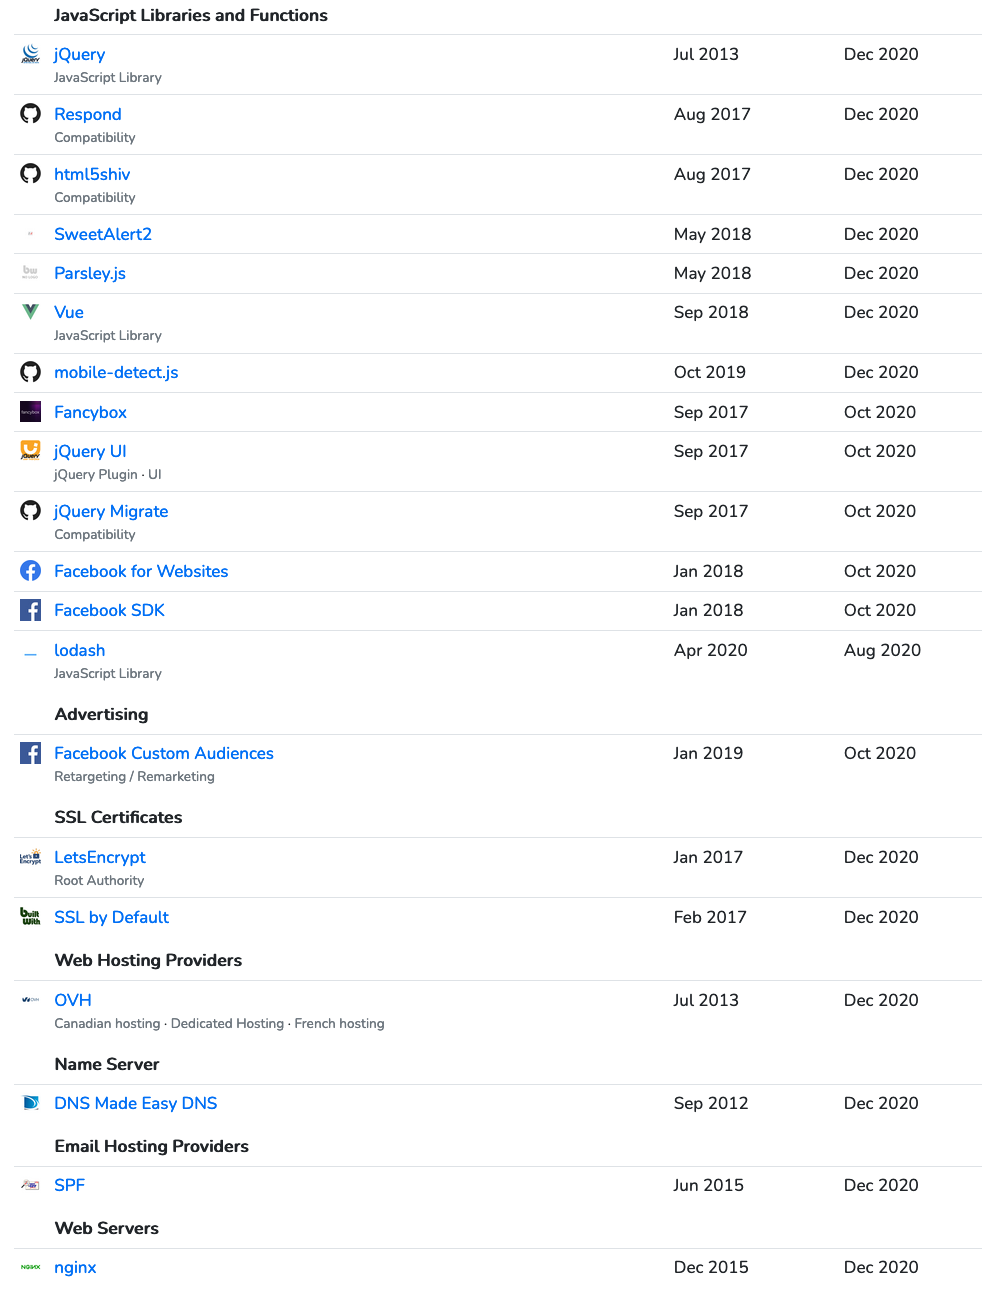
\includegraphics[width=.47\linewidth]{img/builtwith2.png}
 	\caption{BuiltWith result}
\end{figure}



\subsubsection{SecurityHeaders.io}

Another interesting aspect worth analysing are the website's headers. To do that we are going to use \textbf{ \href{https://securityheaders.com/?q=chip7.pt&followRedirects=on}{SecurityHeaders.io}} because it awards the website a grade, and we want to use it as a benchmark value.

\begin{figure}[ht!]
 	\centering
 	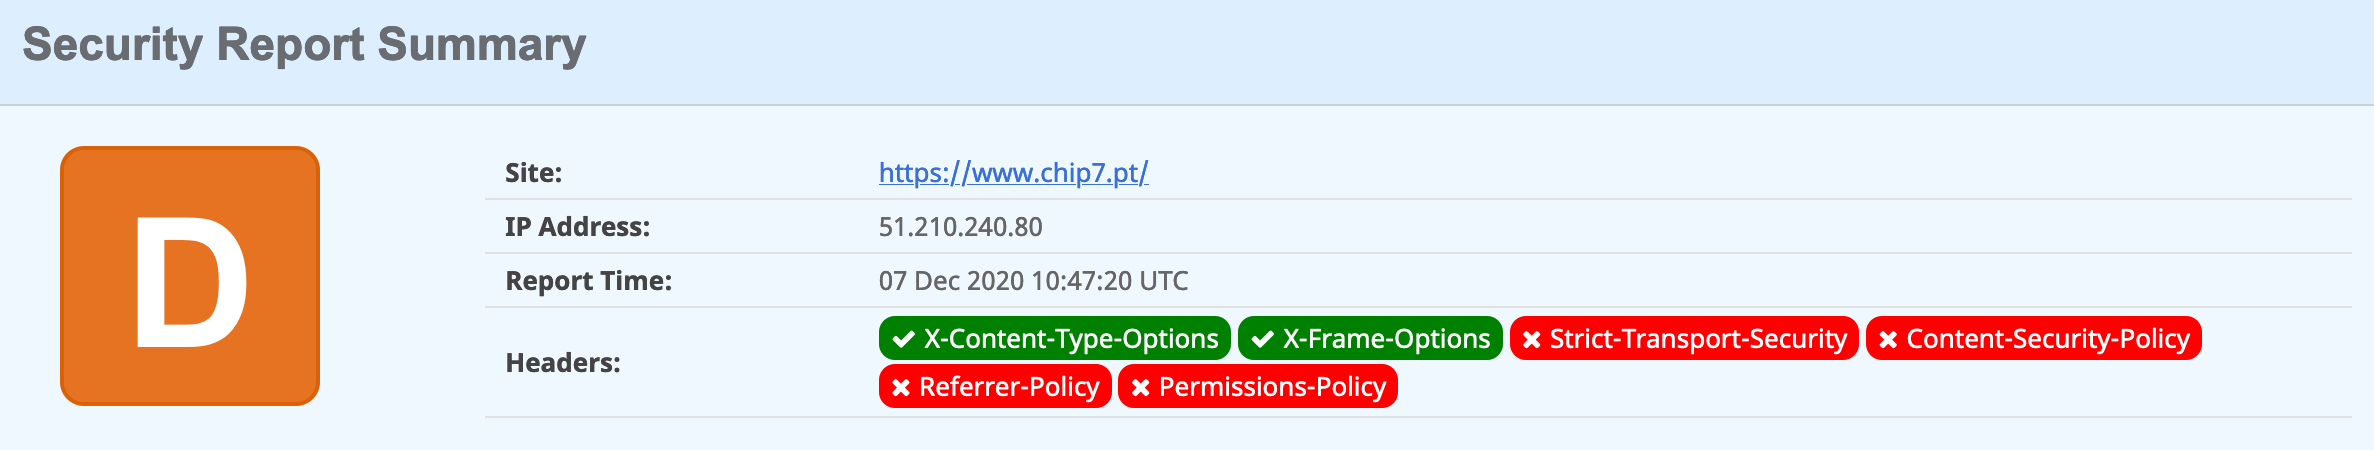
\includegraphics[width=1\linewidth]{img/securityheaders1.png}
 	\caption{Security Headers result}
\end{figure}

As we can see, this website managed a classification of \textbf{D}, which isn't great. This is caused by the lack of 4 security headers which should be implemented:

\begin{itemize}
    \item \textbf{Strict-Transport-Security} - HTTP Strict Transport Security is an excellent feature to support a site and strengthens an implementation of TLS by getting the User Agent to enforce the use of HTTPS. Recommended value "Strict-Transport-Security: max-age=31536000; includeSubDomains".
    \item \textbf{Content-Security-Policy} - Content Security Policy is an effective measure to protect a site from XSS attacks. By whitelisting sources of approved content, it can prevent the browser from loading malicious assets.
    \item \textbf{Referrer-Policy} - Referrer Policy is a new header that allows a site to control how much information the browser includes with navigations away from a document and should be set by all sites.
    \item \textbf{Permissions-Policy} - Permissions Policy is a new header that allows a site to control which features and APIs can be used in the browser.
\end{itemize}

% For more specific informations about the problems in the headers, they can be found in the Report Summary linked before.


\subsection{Farfetch}

\subsubsection{Whois}

For this company we also started by running \textbf{whois} with their domain in order to get more information.

\begin{figure}[ht!]
 	\centering
 	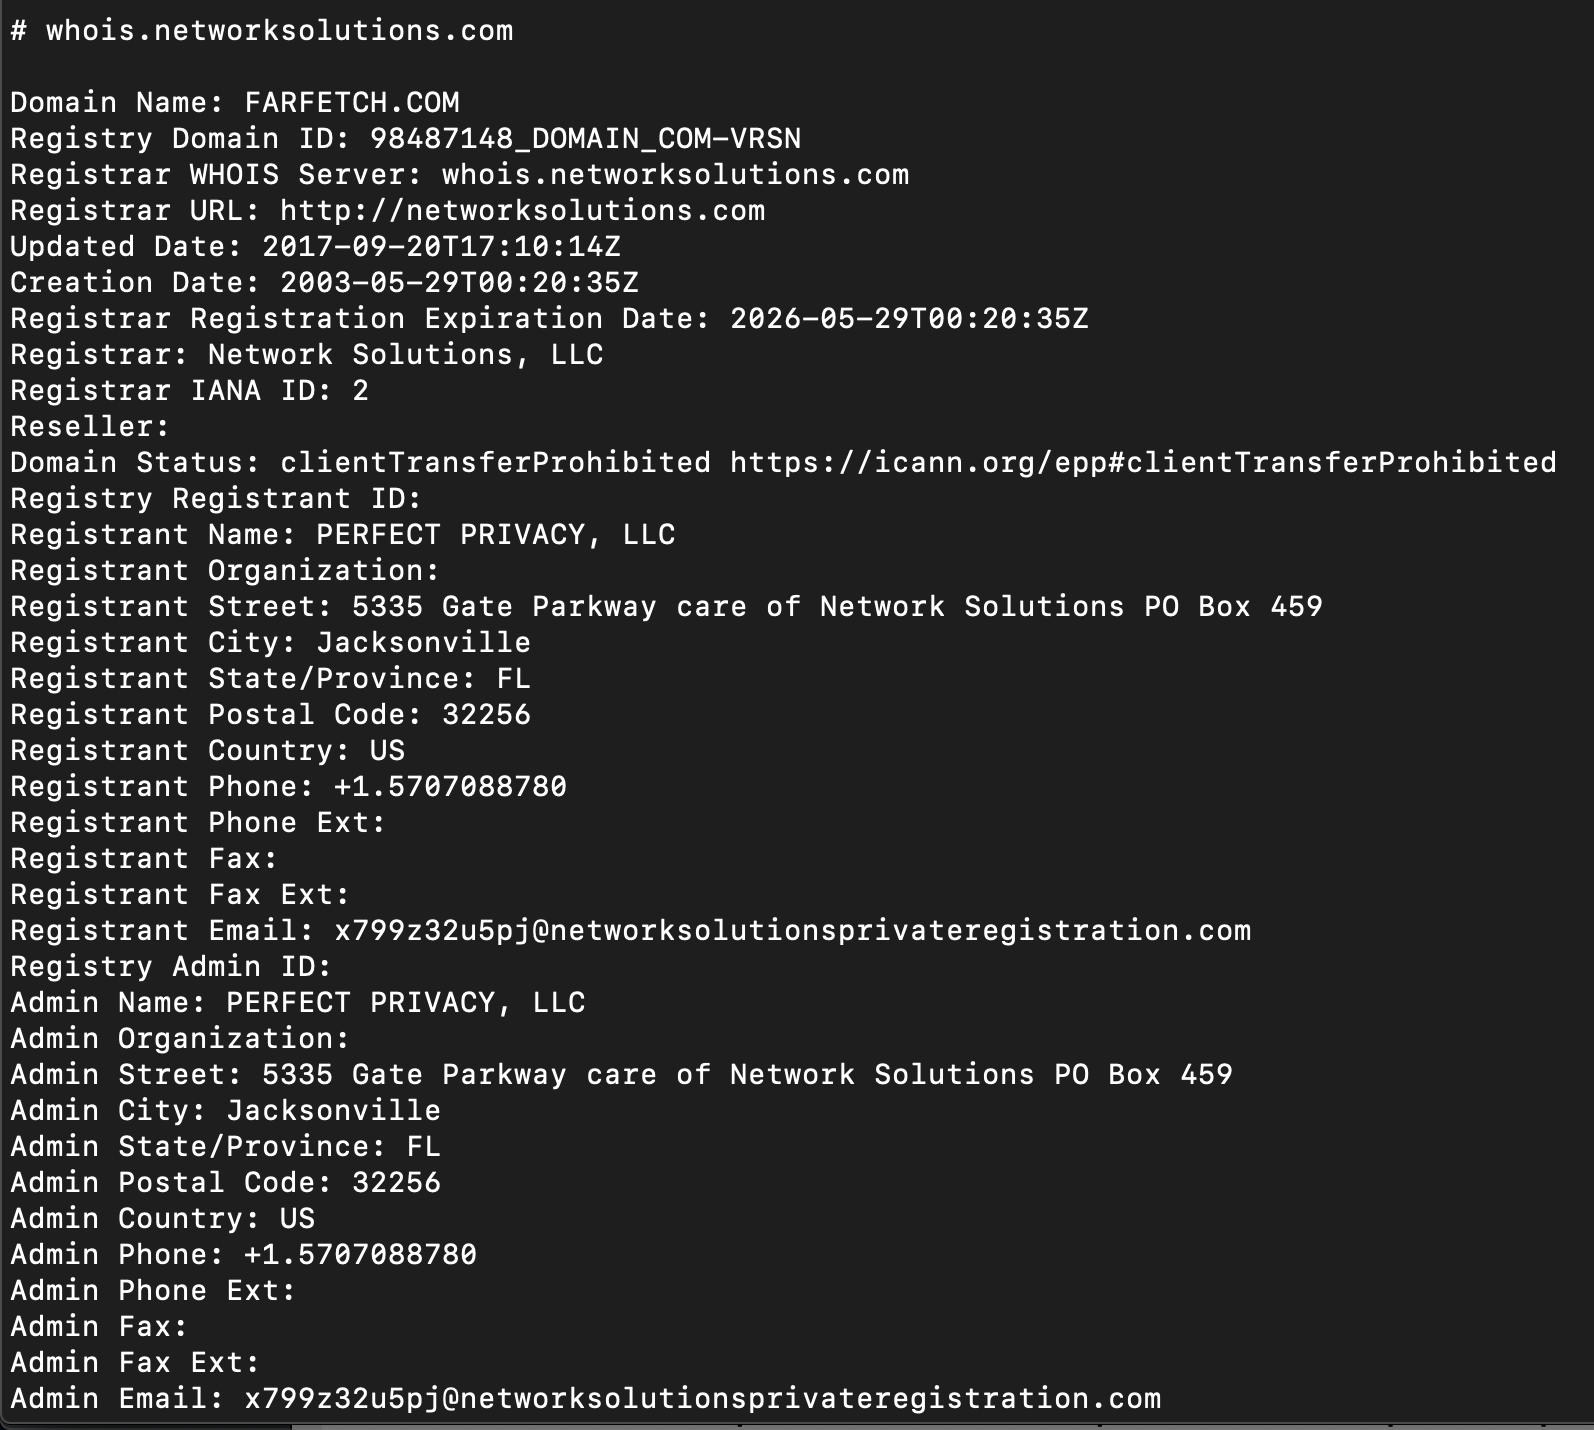
\includegraphics[width=.62\linewidth]{img/whois2.png}
 	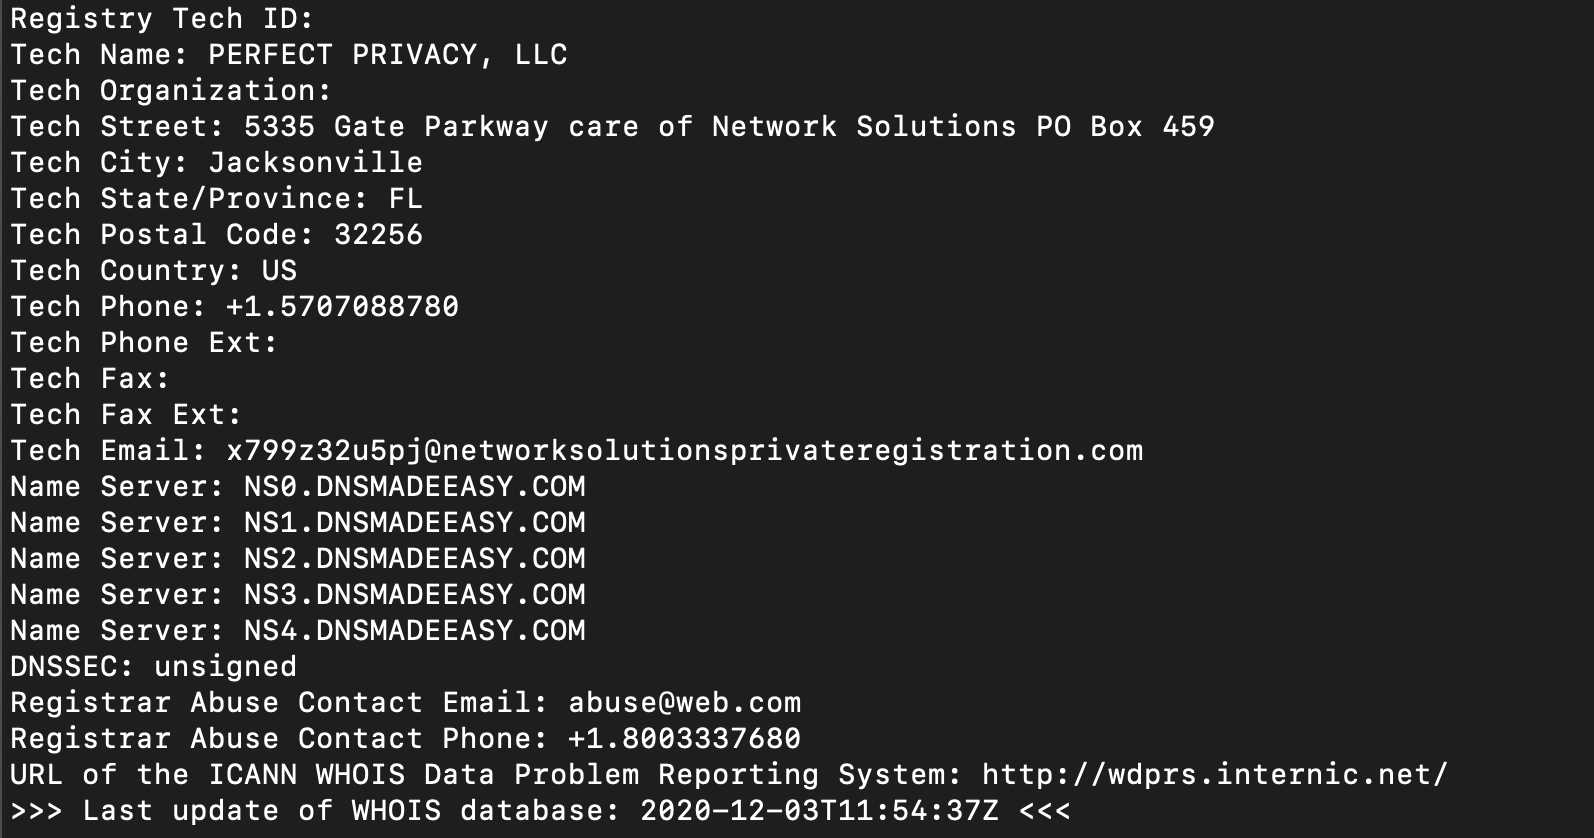
\includegraphics[width=.62\linewidth]{img/whois3.png}
 	\caption{whois result}
\end{figure}


As we can see, despite having more data returned, we obtained less information about the company that we targeted. In this case, they used a company (Perfect Privacy LLC) to act as a Proxy and protect private information. So we haven't got no private email nor an valid address, only a Post-office box, and we also noticed that the expiration date of the domain won't end in the near future (2026). 

\subsubsection{Nslookup \& Whois}
The next step will be, just like with the other company, retrieving the \textbf{IP Address} of the domain, and with that Address trying to know "whois" responsible for it. For the part of fetching the \textbf{IP Address} of the domain, we used \textbf{nslookup}:

\begin{figure}[ht!]
 	\centering
 	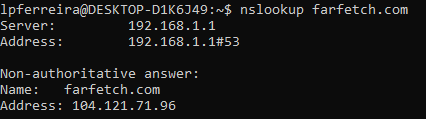
\includegraphics[width=.5\linewidth]{img/nslookupfarfetch.PNG}
 	\caption{nslookup result}
\end{figure}

Having obtained the wanted \textbf{IP Address}, we now query it with \textbf{whois} to get more information:

\begin{figure}[ht!]
 	\centering
 	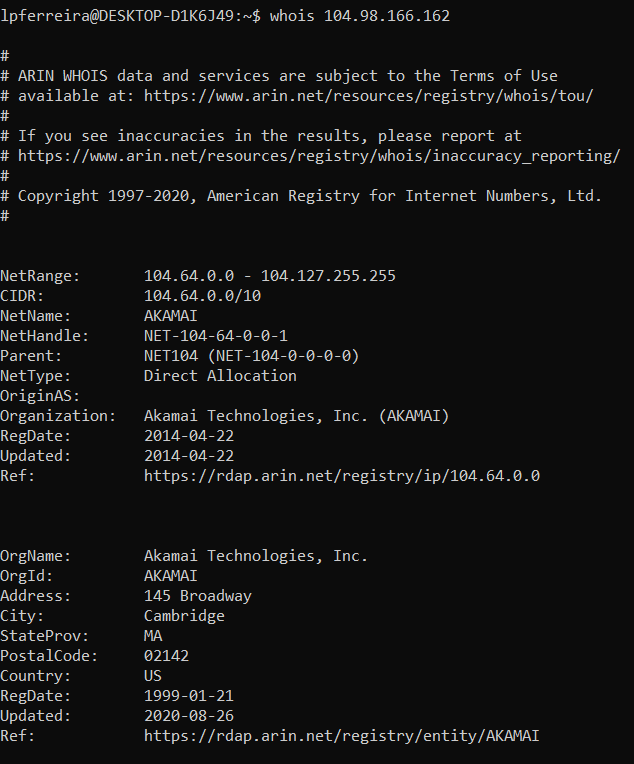
\includegraphics[width=.61\linewidth]{img/whoisfarfetch1.PNG}
 	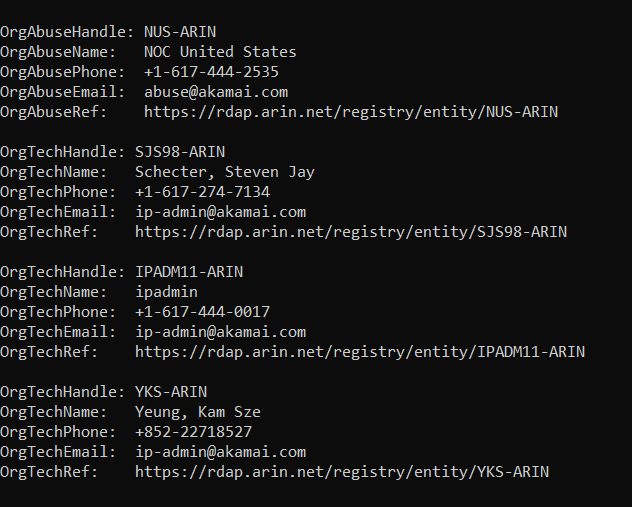
\includegraphics[width=.61\linewidth]{img/whoisfarfetch2.PNG}
 	\caption{whois result}
\end{figure}


Looking at the result we obtained, we discovered that the information is related to \textbf{Akamai}, a global content delivery network (CDN), cybersecurity, and cloud service company, which should be one who's hosting the web pages.

\subsubsection{Job Offers}
Once again, we want to get some information on the technologies and tools used with development of this site. This time, we got some useful information when searching for job offers mainly using a business oriented social network called \textbf{LinkedIn}\cite{linkedin1}.

In that job offer they mention they are searching for someone who has experience in some technologies, those being \texttt{.NET Core}, \texttt{Java}, \texttt{Apache Cassandra}, \texttt{Apache Kafka}, \texttt{RabbitMQ}, \texttt{Neo4j}, \texttt{PostgreSQL}, \texttt{Docker} and \texttt{Kubernetes}. This is some good information to know what is used in their website. Despite this information, \textbf{Farfetch} was careful enough so we couldn't get any versions for that technologies so we could get some vulnerabilities out of them. 


\subsubsection{BuiltWith}

Having got some technologies, we still used \textbf{\href{https://builtwith.com/detailed/farfetch.com/}{BuiltWith}} tool so we can get more information about the technologies implemented on their website. 


%\begin{figure}[ht!]
% 	\centering
% 	\includegraphics[width=.49\linewidth]{img/builtwithfarfetch1.PNG}
% 	\includegraphics[width=.49\linewidth]{img/builtwithfarfetch2.PNG}
% 	\caption{BuiltWith result}
%\end{figure}

This time we got a lot of information in every section of the technology profile, so we choose not to fill pages with prints. But all the information can be accessed \textbf{\href{https://builtwith.com/detailed/farfetch.com/}{here}}.

Just by hovering over all that technology we could notice that a lot of technologies are implemented with the purpose of having a more secure environment. There are plenty of frameworks that are in use, like \textbf{ASP.NET}, \textbf{PHP}, \textbf{Perl} and \textbf{Java}. Just like a lot JavaScript libraries, like \textbf{JQuery}, \textbf{core-js} and \textbf{React}. We can also confirm that \textbf{Akamai} is indeed the web hosting provider and main Content Delivery Network.


\subsubsection{SecurityHeaders.io}

In order to make a comparison with the previous company, we also analysed the headers using \textbf{\href{https://securityheaders.com/?q=farfetch.com&followRedirects=on}{SecurityHeaders.io}}.

\begin{figure}[ht!]
 	\centering
 	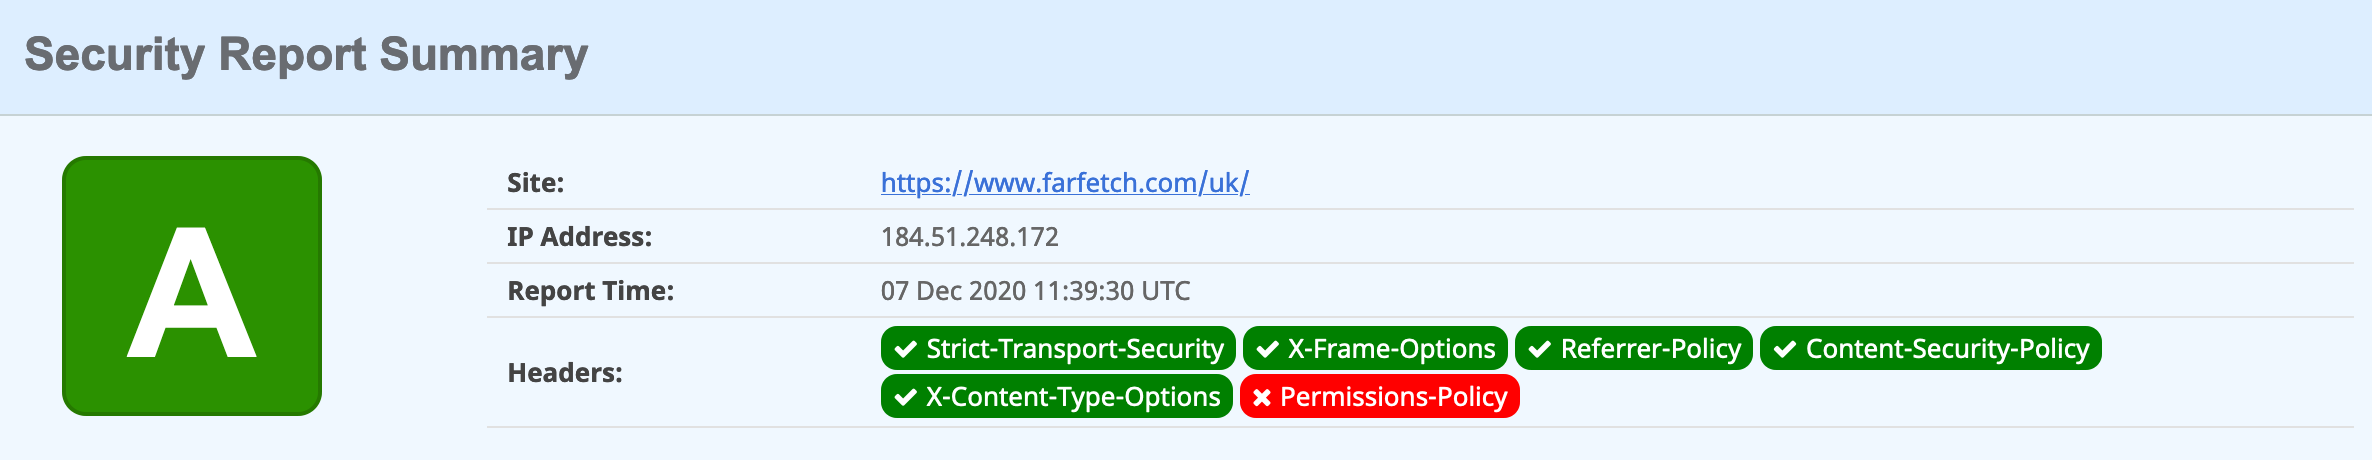
\includegraphics[width=1\linewidth]{img/securityheaders2.png}
 	\caption{Security Headers result}
\end{figure}

As we can see, Farfetch managed to get a score of \textbf{A}, beating the previous score of D. Regarding to these scores we can conclude that Farfetch is more careful with the security of their site. Only having one similar missing header being:

\begin{itemize}
    \item \textbf{Permissions-Policy} - Permissions Policy is a new header that allows a site to control which features and APIs can be used in the browser.
\end{itemize}

\pagebreak